\chapter{Introduction}
\label{ch:intro}

Earthquakes are among the most destructive natural phenomena, and they are also a
remarkable statistical object: their sizes span many orders of magnitude, and small and
large earthquakes obey one simple law, the Gutenberg--Richter law. This thesis studies a
classical mechanical model of an earthquake fault, the Burridge--Knopoff model, and asks
whether its statistics can be understood by mapping it onto a much simpler kind of model,
a \emph{sandpile model}. This first chapter introduces the physical background, defines
how the size of an earthquake is measured, states the Gutenberg--Richter law carefully,
and then describes the two models and the questions this thesis tries to answer.

% ======================================================================
\section{Earthquakes as stick--slip motion}
\label{sec:stickslip}

The outer shell of the Earth is broken into tectonic plates that move relative to each other
at a few centimetres per year. Where two plates meet, they are separated by a \emph{fault}: a
surface along which the rock on one side can slide past the rock on the other side. The two
sides are pressed together, so sliding is resisted by friction.

The simplest picture of how an earthquake happens is Reid's \emph{elastic rebound} theory,
formulated after the 1906 San Francisco earthquake. Far from the fault the plates move
steadily, but near the fault the two sides are held together by friction and do not move.
The rock in between therefore deforms elastically, like a spring that is slowly stretched,
and stores elastic energy. When the shear stress on the fault exceeds what friction can
resist, the fault slips suddenly. The stored elastic energy is released in a few seconds:
part of it is radiated as seismic waves, which are what we feel as an earthquake, and part is
dissipated as heat by friction. After the slip the fault locks again, and the process
repeats.

This alternation of long periods of rest (sticking) and short episodes of fast motion
(slipping) is called \emph{stick--slip motion}. It is familiar from everyday life: a door
hinge that creaks, a violin bow drawn across a string, or chalk squeaking on a blackboard. Two
properties of friction are essential for stick--slip:
\begin{enumerate}[nosep]
  \item \textbf{Static friction is larger than kinetic friction.} A body at rest stays at
    rest until the applied force exceeds a threshold, the maximum static friction force.
    Once it moves, the friction force is smaller.
  \item \textbf{Velocity weakening.} The kinetic friction force decreases as the sliding
    velocity increases. A block that starts to slide therefore experiences less and less
    resistance and accelerates: the motion is unstable.
\end{enumerate}
Both properties will be built into the Burridge--Knopoff model of \cref{sec:bk-intro}.

The time scales involved are extremely different. A large fault such as the San Andreas fault
is loaded at about \SI{3.5}{cm} per year. A large earthquake on it involves a slip of a few
metres, so the time needed to build up the stress released in such an event is roughly
\begin{equation}
  t_{\text{load}} \approx \frac{\SI{3}{m}}{\SI{3.5}{cm/yr}} \approx 90\ \text{years}
  \approx \SI{3e9}{s},
\end{equation}
while the slip itself lasts tens of seconds, $t_{\text{slip}}\approx\SI{30}{s}$. The ratio
$t_{\text{slip}}/t_{\text{load}}\approx 10^{-8}$ is tiny. This \emph{separation of time scales}
between slow loading and fast release will be a central ingredient of everything that follows.

% ======================================================================
\section{Measuring the size of an earthquake}
\label{sec:moment}

\subsection{The seismic moment}

The most physical measure of the size of an earthquake is the \emph{seismic moment}
\begin{equation}
  M_0 = \mu_{\mathrm s}\, A\, \bar D ,
  \label{eq:M0}
\end{equation}
where
\begin{itemize}[nosep]
  \item $\mu_{\mathrm s}$ is the \emph{shear modulus} (rigidity) of the rock, which says how much
    stress is needed to produce a given shear deformation; for crustal rock
    $\mu_{\mathrm s}\approx\SI{3e10}{Pa}$;
  \item $A$ is the \emph{area of the rupture}, the part of the fault surface that slipped;
  \item $\bar D$ is the \emph{average slip}, the relative displacement of the two sides of the
    fault, averaged over the rupture area.
\end{itemize}
The unit of $M_0$ is pascal $\times$ m$^2$ $\times$ m $=$ N\,m. The name ``moment'' comes from the
fact that $M_0$ is the strength of the pair of force couples that represent the earthquake
in seismology; for us it is enough that $M_0$ is proportional to the product of how much area
slipped and how far it slipped.

\begin{example}
\label{ex:moment}
Suppose a rectangular patch of fault \SI{10}{km} long and \SI{10}{km} deep slips by an average
of \SI{1}{m}. Then $A = 10^4\,\text{m}\times10^4\,\text{m} = \SI{e8}{m^2}$ and
\[
  M_0 = (\SI{3e10}{Pa})\times(\SI{e8}{m^2})\times(\SI{1}{m}) = \SI{3e18}{N.m}.
\]
\end{example}

\subsection{The moment magnitude}

Seismic moments range from about $10^{9}$\,N\,m for the smallest recorded earthquakes to about
$10^{23}$\,N\,m for the largest (Chile, 1960). Because this range is so large, a logarithmic scale
is used. The \emph{moment magnitude} is defined as~\cite{HanksKanamori1979}
\begin{equation}
  M_w = \frac{2}{3}\left(\log_{10} M_0 - 9.1\right), \qquad M_0 \text{ in N\,m}.
  \label{eq:Mw}
\end{equation}
The factor $2/3$ and the constant $9.1$ were chosen so that $M_w$ agrees with the older Richter
magnitude scale in the range where both are used. For \cref{ex:moment},
$M_w = \tfrac23(\log_{10}(3\times10^{18}) - 9.1) = \tfrac23(18.48-9.1) \approx 6.3$.

Inverting \cref{eq:Mw} gives $M_0 = 10^{1.5M_w+9.1}$. Increasing the magnitude by one unit
therefore multiplies the moment by $10^{1.5}\approx 32$, and increasing it by two units multiplies
it by $1000$. A magnitude-8 earthquake releases a thousand times more moment than a magnitude-6
earthquake.

\begin{table}[t]
\centering
\caption{The seismic moment and the moment magnitude.}
\label{tab:Mw}
\begin{tabular}{ccl}
\toprule
$M_w$ & $M_0$ [N\,m] & example \\
\midrule
2 & $1.3\times10^{12}$ & smallest events felt by people nearby \\
4 & $1.3\times10^{15}$ & light earthquake, felt widely \\
6 & $1.3\times10^{18}$ & strong earthquake, rupture length $\sim$\SI{10}{km} \\
8 & $1.3\times10^{21}$ & great earthquake, rupture length $\sim$\SI{200}{km} \\
9.5 & $2\times10^{23}$ & Chile 1960, the largest ever recorded \\
\bottomrule
\end{tabular}
\end{table}

% ======================================================================
\section{The Gutenberg--Richter law}
\label{sec:GR}

\subsection{Statement}

Take a catalogue of all earthquakes recorded in some region over some period, and let
$N(\geq M_w)$ be the number of earthquakes whose magnitude is at least $M_w$. Gutenberg and
Richter observed~\cite{GutenbergRichter1944} that, over a wide range of magnitudes,
\begin{equation}
  \log_{10} N(\geq M_w) = a - b\, M_w .
  \label{eq:GR}
\end{equation}
This is the \emph{Gutenberg--Richter law}. Its two parameters are:
\begin{itemize}
  \item The \textbf{$a$-value}. Setting $M_w=0$ gives $N(\geq 0)=10^{a}$, so $a$ measures the
    overall level of seismic activity of the region (and depends on how long and how large an
    area was observed). It contains no information about the relative frequency of small and large
    events.
  \item The \textbf{$b$-value}. It is the slope of the straight line in a plot of $\log_{10}N$
    against $M_w$. If the magnitude increases by one unit, $N$ is divided by $10^{b}$. In almost all
    tectonic regions $b\approx 1$: \emph{for each unit of magnitude there are about ten times fewer
    earthquakes}.
\end{itemize}

\begin{example}
If a region has 1000 earthquakes of magnitude 3 or more per year and $b=1$, it has on average
100 of magnitude 4 or more, 10 of magnitude 5 or more, and one of magnitude 6 or more per year.
\end{example}

\subsection{From magnitudes to a power law of the moment}

The Gutenberg--Richter law is written with magnitudes, which are logarithms. It is very useful to
rewrite it in terms of the physical size $M_0$. Substituting \cref{eq:Mw} into \cref{eq:GR}:
\begin{align}
  \log_{10} N &= a - b\cdot\tfrac23\left(\log_{10} M_0 - 9.1\right)
             = \underbrace{\left(a + \tfrac23\, 9.1\, b\right)}_{\text{constant}} - \tfrac{2b}{3}\log_{10} M_0 , \\
  N(\geq M_0) &= C\, M_0^{-2b/3} ,
  \label{eq:GR-moment-cum}
\end{align}
where $C$ is a constant. So the number of earthquakes with moment larger than $M_0$ decays as a
\emph{power} of $M_0$, with exponent $2b/3\approx 2/3$.

$N(\geq M_0)$ is a \emph{cumulative} quantity: it counts all events above a threshold. Often one wants
the \emph{probability density} $P(M_0)$, defined so that $P(M_0)\,\dd M_0$ is the fraction of
earthquakes with moment between $M_0$ and $M_0+\dd M_0$. The number of events in that interval is
$N(\geq M_0) - N(\geq M_0+\dd M_0) = -\frac{\dd N}{\dd M_0}\dd M_0$, so
\begin{equation}
  P(M_0) = -\frac{1}{N_{\text{tot}}}\frac{\dd N(\geq M_0)}{\dd M_0}
         = \frac{C}{N_{\text{tot}}}\,\frac{2b}{3}\, M_0^{-2b/3-1}
         \;\propto\; M_0^{-\tau}, \qquad \tau = 1 + \frac{2b}{3} .
  \label{eq:GR-density}
\end{equation}
With $b=1$ this gives $\tau = 5/3\approx1.67$. The two forms of the law are shown in
\cref{fig:GR}. On a logarithmic plot both are straight lines: the cumulative count against $M_w$
with slope $-b$, and the density against $M_0$ with slope $-\tau$.

\begin{figure}[t]
  \centering
  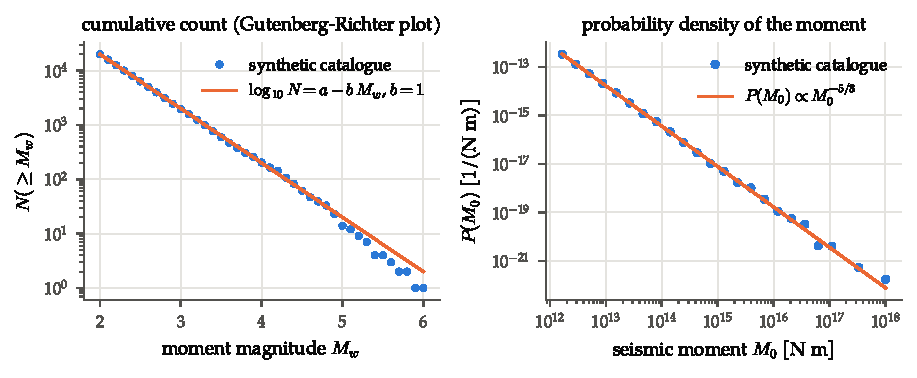
\includegraphics[width=\linewidth]{soc/gutenberg_richter.pdf}
  \caption{The two forms of the Gutenberg--Richter law, illustrated with a synthetic catalogue of
  $20\,000$ events generated with $b=1$ (not real data). Left: number of events with magnitude at
  least $M_w$, on a logarithmic vertical axis; the slope is $-b$. Right: the same events
  as a probability density of the seismic moment, on logarithmic axes; the slope is $-\tau=-5/3$.
  The scatter at the largest sizes is the statistical noise of the few largest events.}
  \label{fig:GR}
\end{figure}

\subsection{What the law means}

A probability density of the form $P(x)\propto x^{-\tau}$ is called a \emph{power law}, and $\tau$ is
its \emph{exponent}. Chapter~\ref{ch:soc} explains in detail why power laws are special. The main
point can be stated already: a power law has \emph{no characteristic scale}. There is no
``typical'' earthquake size, in the sense in which there is a typical height of a person; there
are simply fewer large events than small ones, in a fixed ratio for every factor of size.

A second consequence concerns which events dominate. The total moment released by all earthquakes
with moments between $M_{\min}$ and $M_{\max}$ is proportional to
\begin{equation}
  \int_{M_{\min}}^{M_{\max}} M_0\, P(M_0)\, \dd M_0 \;\propto\; \int_{M_{\min}}^{M_{\max}} M_0^{1-\tau}\,\dd M_0
  = \frac{M_{\max}^{2-\tau} - M_{\min}^{2-\tau}}{2-\tau} \;\approx\; \frac{M_{\max}^{1/3}}{1/3}
\end{equation}
for $\tau = 5/3$ and $M_{\max}\gg M_{\min}$. The result depends on the \emph{largest} events and hardly
at all on the smallest. Although small earthquakes are far more numerous, most of the slip on a fault
is accomplished by its few largest earthquakes.

\subsection{The magnitude used by Carlson and Langer}

The papers on the Burridge--Knopoff model that this thesis builds on~\cite{CarlsonLanger1989,Carlson1991}
use a different, simpler magnitude: the natural logarithm of the model's moment,
\begin{equation}
  \mu = \ln M .
\end{equation}
(Here $M$ is the moment of the model, defined in Chapter~4; $\mu$ is unrelated to the shear
modulus $\mu_{\mathrm s}$.) They write their results as a frequency density in $\mu$,
$\mathcal R(\mu)\propto e^{-b\mu}$, and call $b$ the $b$-value. To relate this to a power law in $M$,
note that the same events are counted whether we use $\mu$ or $M$:
$\mathcal R(\mu)\,\dd\mu = P(M)\,\dd M$. Since $\dd\mu = \dd M/M$,
\begin{equation}
  P(M) = \mathcal R(\mu)\frac{\dd\mu}{\dd M} = \frac{e^{-b\ln M}}{M} = M^{-(1+b)} .
  \label{eq:CL-b-tau}
\end{equation}
So in Carlson and Langer's language, ``$b=1$, consistent with Gutenberg--Richter'' means a moment density
$P(M)\propto M^{-2}$, i.e.\ $\tau = 2$, and \emph{not} the $\tau=5/3$ of \cref{eq:GR-density}. The two
$b$-values differ because the magnitudes are defined differently (natural logarithm and no factor
$2/3$). This difference must be kept in mind whenever results of the model are compared with
seismological data or with the exponents of sandpile models.

% ======================================================================
\section{Two kinds of models}
\label{sec:models}

Real faults are three-dimensional, heterogeneous, and only partly observable. To understand
\emph{why} the Gutenberg--Richter law holds, physicists have studied models that are deliberately
much simpler than a real fault but keep what is believed to be essential. Two families of models
are central to this thesis.

\subsection{The Burridge--Knopoff model}
\label{sec:bk-intro}

In 1967 Burridge and Knopoff~\cite{BurridgeKnopoff1967} proposed a mechanical model of a fault made of
blocks and springs (\cref{fig:bk-sketch}). A chain of $N$ identical blocks of mass $m$ rests on a rough,
fixed surface, which represents one side of the fault. Each block is connected
\begin{itemize}[nosep]
  \item to its two neighbours by \emph{coupling springs} of spring constant $k_c$, which represent the
    elastic stiffness of the rock along the fault;
  \item to a rigid upper plate by a \emph{pulling spring} of spring constant $k_p$, which represents the
    elastic connection of the fault zone to the far-away part of the moving plate.
\end{itemize}
The upper plate moves at a constant, very small velocity $v$. Between each block and the surface acts
a friction force with the stick--slip properties of \cref{sec:stickslip}: a block stays stuck until the
total spring force on it exceeds the maximum static friction $F_0$, and then slides with a kinetic
friction force that decreases with its velocity.

\begin{figure}[t]
\centering
\begin{tikzpicture}[x=10mm,y=10mm,>={Stealth[length=2mm]}]
  % floor
  \fill[pattern=north east lines,pattern color=ink2!60] (-0.4,-0.25) rectangle (10.4,0);
  \draw[ink2,thick] (-0.4,0) -- (10.4,0);
  \node[ink2,font=\footnotesize,anchor=west] at (10.5,-0.12) {fixed rough surface};
  % plate
  \fill[cblue!12] (-0.4,2.2) rectangle (10.4,2.6);
  \draw[ink2] (-0.4,2.2) rectangle (10.4,2.6);
  \node[font=\footnotesize,anchor=west] at (10.5,2.4) {plate, velocity $v$};
  \draw[->,cblueD,thick] (8.6,2.85) -- (10.0,2.85);
  % blocks
  \foreach \i in {0,...,4} {
    \pgfmathsetmacro\x{0.6+2.2*\i}
    \draw[ink2,fill=corange!20] (\x,0) rectangle (\x+1.0,0.8);
    \node[font=\footnotesize] at (\x+0.5,0.4) {$m$};
    % pulling spring
    \draw[ink2,decorate,decoration={zigzag,segment length=2.2mm,amplitude=1mm}] (\x+0.5,0.8) -- (\x+0.5,2.2);
  }
  \foreach \i in {0,...,3} {
    \pgfmathsetmacro\x{1.6+2.2*\i}
    \draw[ink2,decorate,decoration={zigzag,segment length=2.2mm,amplitude=1mm}] (\x,0.4) -- (\x+1.2,0.4);
  }
  \node[font=\footnotesize,ink2] at (2.2,0.75) {$k_c$};
  \node[font=\footnotesize,ink2,anchor=west] at (1.15,1.5) {$k_p$};
  \node[font=\footnotesize,ink2] at (5.5,-0.55) {friction $F(\dot x)$ between each block and the surface ($\dot x$: velocity of the block)};
\end{tikzpicture}
\caption{The Burridge--Knopoff model: blocks of mass $m$ connected to each other by coupling springs
$k_c$ and to a slowly moving plate by pulling springs $k_p$, sliding with stick--slip friction on a
fixed surface.}
\label{fig:bk-sketch}
\end{figure}

The dynamics is simple to state. The pulling springs are stretched slowly and uniformly by the plate.
When one block reaches the friction threshold, it slips; its motion changes the force on its neighbours
through the coupling springs, and they may slip too. The resulting cascade is a model earthquake. Its
size is measured by the moment, the sum of the displacements of all the blocks that moved, in close
analogy with \cref{eq:M0}.

Carlson and Langer~\cite{CarlsonLanger1989} studied this model in detail and found that, without any
randomness in the model, it produces a broad distribution of event sizes that is consistent with the
Gutenberg--Richter law for small and intermediate events, together with an excess of very large
events. The model and these results are the subject of Chapter~4.

\subsection{Sandpile models}

At almost the same time, Bak, Tang and Wiesenfeld~\cite{BTW1987,BTW1988} introduced a much simpler kind of
model, the \emph{sandpile model}. Grains are dropped one by one onto a lattice; when the number of grains
at a site exceeds a threshold, the site ``topples'' and passes grains to its neighbours, which may topple
in turn. The sandpile has no masses, velocities or forces, only integers and a rule. Yet it shows avalanches
of all sizes with power-law distributions, and it reaches this state by itself, without any parameter
being tuned. Bak, Tang and Wiesenfeld called this behaviour \emph{self-organized criticality} and proposed
that it explains the Gutenberg--Richter law, among many other power laws in nature. Chapter~\ref{ch:soc}
introduces these ideas in detail.

The analogy between the two kinds of models is clear: in both, a quantity (stress, grains) is loaded slowly,
released when a local threshold is exceeded, and redistributed to neighbours, producing avalanches. In 1992
Olami, Feder and Christensen~\cite{OFC1992} made the analogy precise for a two-dimensional version of the
Burridge--Knopoff model, by removing the inertia of the blocks and turning the model into a sandpile-like
automaton with continuous variables.

% ======================================================================
\section{This project}
\label{sec:project}

\subsection{The question}

The central question of this thesis is:
\begin{quote}
\emph{Can the statistics of the one-dimensional Burridge--Knopoff model be understood by mapping it onto a
sandpile model? If so, what are its critical exponents; if not, what exactly is lost in the mapping?}
\end{quote}
The mapping is attractive because sandpile models are far easier to simulate and, in some cases, to solve
exactly. But the Burridge--Knopoff model contains something that a sandpile does not: inertia. A slipping
block has kinetic energy, and Carlson and Langer showed that the largest events of the model are driven by
pulses of slip that grow as they propagate along the chain. It is therefore not obvious that a sandpile
can capture all of the model's behaviour.

\subsection{History of the project}

This thesis revives an earlier attempt at the same question. That attempt stalled at the first step: the
numerical simulations could not reproduce the size distributions published by Carlson and
Langer in 1989~\cite{CarlsonLanger1989}. Two reasons emerged. First, the 1989 paper was based on relatively
short simulations, and its later companion paper by Carlson, Langer, Shaw and Tang (1991)~\cite{Carlson1991}
uses a modified friction law and a different limit of the loading speed, with noticeably different results.
Second, a careful review of the old simulation code, carried out for this thesis, found several errors in
the numerical integration, in the boundary conditions and in the units of the parameters. The present work
therefore starts again from a clean, tested implementation.

\subsection{Aims}

The aims of this thesis are:
\begin{enumerate}[nosep]
  \item to review the theory of self-organized criticality and of sandpile models at the level needed for the
    project;
  \item to review the analysis of the Burridge--Knopoff model by Carlson and collaborators, and in particular
    to understand the differences between the 1989 and 1991 papers;
  \item to implement the Burridge--Knopoff model and the relevant sandpile models, and to verify the
    implementations against exactly known results;
  \item to reproduce the published results of the Burridge--Knopoff model;
  \item to derive the mapping from the Burridge--Knopoff model to a sandpile model, and to test by simulation
    where it holds and where it fails;
  \item to develop an approximate theory (of mean-field or branching-process type) for the exponents of the
    mapped model and to compare it with simulations.
\end{enumerate}

\subsection{Structure of the thesis}

Chapter~\ref{ch:soc} introduces power laws, critical phenomena and self-organized criticality, and studies the
Bak--Tang--Wiesenfeld sandpile in one and two dimensions, including an exact solution in one dimension.
Chapter~3 discusses how exponents are measured reliably from finite data. Chapter~4 presents the
Burridge--Knopoff model and the work of Carlson and collaborators. Chapter~5 derives the mapping to a sandpile
model. Chapter~6 describes the numerical methods and how they were validated, Chapter~7 presents the results,
Chapter~8 the approximate theory, and Chapter~9 summarises the conclusions.
